%Este trabalho está licenciado sob a Licença Atribuição-CompartilhaIgual 4.0 Internacional Creative Commons. Para visualizar uma cópia desta licença, visite http://creativecommons.org/licenses/by-sa/4.0/deed.pt_BR ou mande uma carta para Creative Commons, PO Box 1866, Mountain View, CA 94042, USA.

\chapter{Método de elementos finitos em 1D}\label{cap_mef1d}
\thispagestyle{fancy}

\section{Interpolação e projeção}\label{cap_mef1d_sec_interproj}

Seja dado um intervalo $I = [x_0, x_1]\subset\mathbb{R}$, $x_0\neq x_1$. O \hlemph{espaço vetorial das funções lineares} em $I$ é definido por
\begin{equation}\hleq
  P_1(I) := \{v: ~v(x)=c_0+c_1x,~x\in I,~c_0,c_1\in\mathbb{R}\}.
\end{equation}
Observamos que dado $v\in P_1(I)$, temos que $v$ é unicamente determinada pelos valores
\begin{equation}
  \begin{aligned}
    &\alpha_0 = v(x_0),\\
    &\alpha_1 = v(x_1).
  \end{aligned}
\end{equation}
Como consequência, existe exatamente uma única função $v\in P_1(I)$ para quaisquer dados valores $\alpha_0$ e $\alpha_1$. Desta observação, introduzimos a chamada \hlemph{base nodal} (base lagrangiana\footnote{Consulte mais em \href{https://notaspedrok.com.br/notas/MatematicaNumericaI/cap_interp_sec_lagrange.html}{Notas de Aula: Matemática Numérica I: Interpolação de Lagrange}.}) $\{\varphi_0, \varphi_1\}$ para $P_1(I)$, definida por
\begin{equation}\hleq
  \varphi_j(x_i) = \left\{
    \begin{array}{ll}
      1 &, i=j,\\
      0 &, i\neq j
    \end{array}
\right.,
\end{equation}
com $i,j=0, 1$. Consulte a Figura~\ref{fig:p1_0}.

\begin{figure}[H]
  \centering
  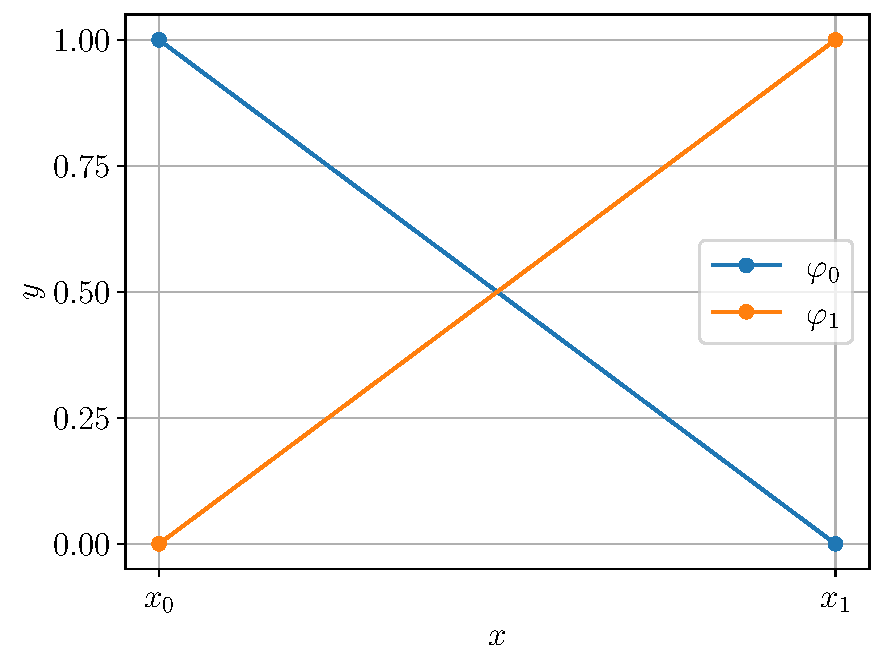
\includegraphics[width=0.7\textwidth]{./cap_mef1d/dados/fig_p1_0/fig}
  \caption{Base nodal para o espaço $P_1([x_0, x_1])$.}
  \label{fig:p1_0}
\end{figure}

Com esta base, toda função $v\in P_1(I)$ pode ser escrita como uma combinação linear das funções $\varphi_0$ e $\varphi_1$ com coeficientes $\alpha_0$ e $\alpha_1$ (\hlemph{graus de liberdade}), i.e.
\begin{equation}\hleq
  v(x) = \alpha_0\varphi_0(x) + \alpha_1\varphi_1(x).
\end{equation}
Além disso, observamos que
\begin{align}
  &\varphi_0(x) = \frac{x-x_1}{x_0-x_1},\\
  &\varphi_1(x) = \frac{x-x_0}{x_1-x_0}.
\end{align}



Uma extensão do espaço $P_1(I)$ é o \hlemph{espaço das funções lineares por partes}. Dado $I = [l_0, l_1]$, $l_0\neq l_1$, consideremos uma partição (\hlemph{malha}) de $I$ com $n+1$ pontos
\begin{equation}
  \mathcal{I} = \{l_0=x_0, x_1, \dotsc, x_n=l_1\}
\end{equation}
e, portanto, com $n$ subintervalos $I_i=[x_{i-1}, x_{i}]$ de comprimento (\hlemph{tamanho da malha}) $h_i = x_i-x_{i-1}$, $i=1, 2, \dotsc, n$. Na malha $\mathcal{I}$ definimos o seguinte \emph{espaço das funções lineares por partes}
\begin{equation}\hleq
  V_h := \{v:~v\in C^0(\mathcal{I}),~v|_{I_i}\in P_1(I_i),~i=1,2,\dotsc,n\}.
\end{equation}
Observamos que \hl{toda função $v\in V_h$ é unicamente determinada por seus valores nodais $\{\alpha_i = v(x_i)\}_{i=0}^n$}. Reciprocamente, \hl{todo conjunto de valores nodas $\{\alpha_i\}_{i=0}^n$ determina unicamente uma função $v\in V_h$}. Desta observação, temos que os \hlemph{valores nodais determinam os graus de liberdade} com a base nodal $\{\varphi_j\}_{j=0}^n$ para $V_h$ definida por
\begin{equation}\hleq
  \varphi_j(x_i) = \left\{
    \begin{array}{ll}
      1 &, i=j,\\
      0 &, i\neq j
    \end{array}
\right.,
\end{equation}
com $i,j=0,1,\dotsc,n$. Ou seja, temos que
\begin{equation}\hleq
    v(x) = \sum_{j=0}^{n}\alpha_j\phi_j(x).
\end{equation}
Podemos verificar que
\begin{equation}
  \varphi_i(x) = \left\{
    \begin{array}{ll}
      (x-x_{i-1})/h_i &, x\in I_i,\\
      (x_{i+1}-x)/h_{i+1} &, x\in I_{i+1},\\
      0 &, \text{noutros casos}
    \end{array}
\right.
\end{equation}
consulte, Figura~\ref{fig:baselinear}. É notável que $\varphi_i(x)$ tem suporte compacto $I_i\cup I_{i+1}$.

\begin{figure}[h!]
  \centering
  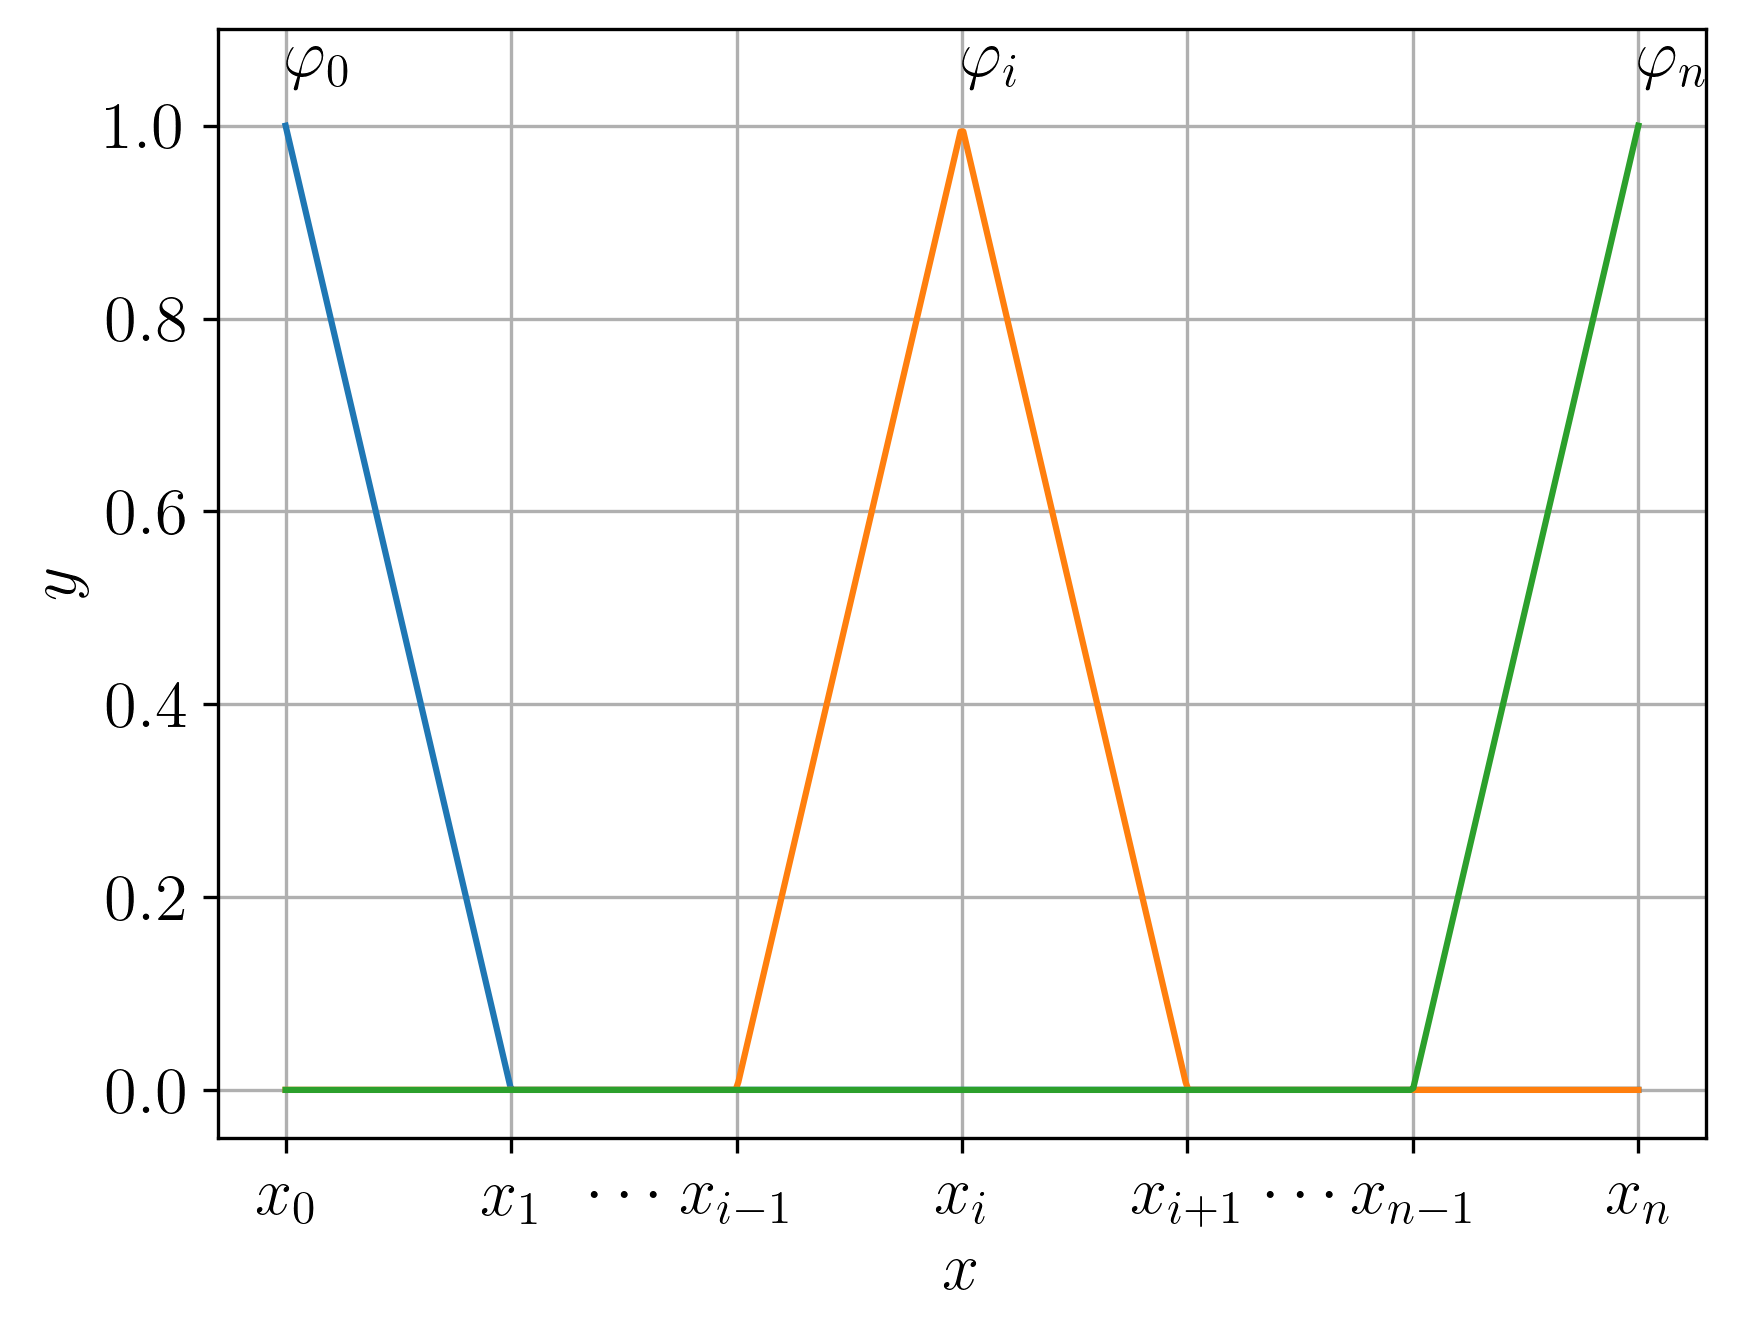
\includegraphics[width=0.7\textwidth]{./cap_mef1d/dados/fig_baselinear/fig}
  \caption{Base nodal para o espaço das funções lineares por parte.}
  \label{fig:baselinear}
\end{figure}

\subsection{Interpolação}
[[tag:revisar]]

\hl{Interpolação é uma técnica de aproximação de funções}. Dada uma função contínua $f$ em $I=[l_0, l_1]$, definimos o \hlemph{operador de interpolação linear} $\pi: C^0(I)\to V_h$ por
\begin{equation}\hleq
  \pi f (x) = \sum_{j=0}^{n}f(x_j)\varphi_j(x)
\end{equation}
Observamos que $\pi f$ é igual a $f$ nos nodos $x_j$, $j=0, 1, 2, \dotsc, n$. 

\begin{ex}\label{ex:mef1d_interp_lin}
  A Figura~\ref{fig:ex_mef1d_interp_lin} ilustra a interpolação da função $f(x)=3\sen(2\pi x)$ no espaço de elementos finitos $V_h$ das funções lineares por partes com $5$ células.

  \begin{figure}[H]
    \centering
    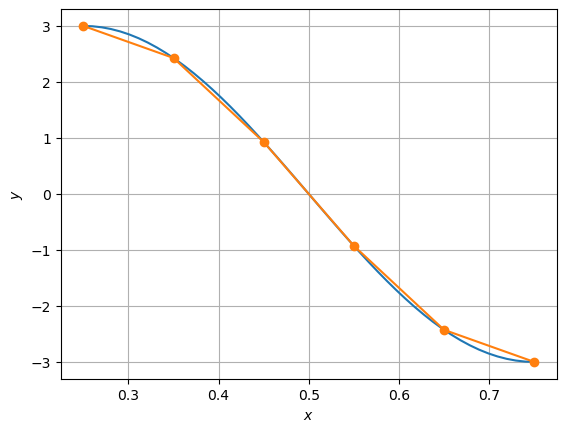
\includegraphics[width=0.8\textwidth]{./cap_mef1d/dados/ex_mef1d_interp_lin/fig}
    \caption{Interpolação linear de $f(x)=3\sen(2\pi x)$ no espaço de elementos finitos $V$.}
    \label{fig:ex_mef1d_interp_lin}
  \end{figure}


\begin{lstlisting}[caption=mef1d\_interp\_lin]
from dolfinx import fem, mesh
import ufl
import numpy as np
from mpi4py import MPI
import matplotlib.pyplot as plt

# malha
l0 = 0.25
l1 = 0.75
domain = mesh.create_interval(MPI.COMM_WORLD,
                              nx = 5,
                              points = [l0, l1])
x = ufl.SpatialCoordinate(domain)

# espaço
V = fem.FunctionSpace(domain, ('P', 1))

# fun
def fun(x, mod):
    return 3.*mod.sin(2.*mod.pi*x)

x = ufl.SpatialCoordinate(domain)
f_expr = fem.Expression(fun(x[0], ufl),
                        V.element.interpolation_points())

# interpolação
pif = fem.Function(V)
pif.interpolate(f_expr)
\end{lstlisting}
\end{ex}

Agora, vamos buscar medir o erro de interpolação, i.e. $f - \pi f$. Para tanto, podemos usar a norma $L^2$ definida por
\begin{equation}
  \|v\|_{L^2(I)} = \left(\int_I v^2\, dx\right)^{1/2}.
\end{equation}
Lembramos que valem a \pmb{desigualdade triangular}\index{desigualdade!triangular}
\begin{equation}
  \|v+w\|_{L^2(I)} \leq \|v\|_{L^2(I)} +  \|w\|_{L^2(I)}
\end{equation}
e a \pmb{desigualdade de Cauchy-Schwarz}\index{desigualdade!de Cauchy-Schwarz}\footnote{Também conhecida como desigualdade de Cauchy–Bunyakovsky–Schwarz. Augustin-Louis Cauchy, 1789 - 1857, matemático francês. Viktor Yakovlevich Bunyakovsky, 1804 - 1889, matemático Russo. Karl Hermann Amandus Schwarz, 1843 - 1921, matemático alemão.}
\begin{equation}\label{eq:Cauchy-Schwarz}
  \int_I vw\,dx \leq \|v\|_{L^2(I)}\|w\|_{L^2(I)},
\end{equation}
para qualquer funções $v,w\in L^2(I)$.

\begin{prop}\normalfont(Erro da interpolação linear)\label{prop:interp_lin}
  O interpolador $\pi f:C^0(I)\to P_1(I)$ satisfaz as estimativas
  \begin{align}
    \|f-\pi f\|_{L^2(I)} &\leq Ch^2\|f''\|_{L^2(I)},\\
    \|(f-\pi f)'\|_{L^2(I)} &\leq Ch\|f''\|_{L^2(I)},
  \end{align}
onde $C$ é uma constante e $h=x_1-x_0$.
\end{prop}
\begin{dem}
  Denotemos o erro de interpolação por $e = f - \pi f$. Do teorema fundamental do cálculo, temos
  \begin{equation}
    e(y) = e(x_0) + \int_{x_0}^y e'(x)\,dx,
  \end{equation}
onde $e(x_0)=f(x_0)-\pi f(x_0) = 0$. Daí, usando a desigualdade de Cauchy-Schwarz~\eqref{eq:Cauchy-Schwarz}, temos
\begin{align}
  e(y) &= \int_{x_0}^y e'\,dx\\
       &\leq \int_{x_0}^y |e'|\,dx\\
       &\leq \int_{I} 1\cdot |e'|\,dx\\
       &\leq \left(\int_{I} 1^2\,dx\right)^{1/2} \left(\int_{I} e'^2\,dx\right)^{1/2}\\
       &= h^{1/2}\left(\int_{I} e'^2\,dx\right)^{1/2},
\end{align}
donde
\begin{equation}
  e(y)^2 \leq h\int_I e'^2\,dx = h\|e'\|_{L^2(I)}^2.
\end{equation}
Então, integrando em $I$ obtemos
\begin{equation}
  \|e\|_{L^2(I)}^2 = \int_I e^2(y)\,dy \leq \int_I h\|e'\|_{L^2(I)}^2\,dy = h^2\|e'\|_{L^2(I)}^2,
\end{equation}
ou seja, temos a seguinte desigualdade
\begin{equation}\label{eq:prop_pif_0}
  \|e\|_{L^2(I)} \leq h\|e'\|_{L^2(I)}.
\end{equation}

Agora, observando que $e(x_0)=e(x_1)=0$, o \pmb{teorema de Rolle}\index{teorema!de Rolle}\footnote{Michel Rolle, 1652 - 1719, matemático francês.} garante a existência de um ponto $\tilde{x}\in I$ tal que $e'(\tilde{x})=0$, donde do teorema fundamental do cálculo e da desigualdade de Cauchy-Schwarz, segue
\begin{align}
  e'(y) &= e'(\tilde{x}) + \int_{\tilde{x}}^y e''\,dx \\
        &= \int_{\tilde{x}}^y e''\,dx\\
        &\leq \int_{I}1\cdot |e''|\,dx\\
        &\leq h^{1/2}\left(\int_I e''^2\right)^{1/2}.
\end{align}
Então, integrando em $I$, obtemos
\begin{equation}\label{eq:prop_pif_1}
  \|e'\|_{L^2(I)}^2 \leq h^2\|e''\|_{L^2(I)}^2,
\end{equation}
a qual, observando que $e'' = f''$, equivale a segunda estimativa procurada, i.e.
\begin{equation}
  \|(f-\pi f)'\|_{L^2(I)} \leq C h \|f''\|_{L^2(I)}.
\end{equation}
Por fim, de \eqref{eq:prop_pif_1} e de \eqref{eq:prop_pif_0}, obtemos a primeira estimativa desejada
\begin{equation}
  \|f - \pi f\|_{L^2(I)} \leq C h^2 \|f''\|_{L^2(I)}.
\end{equation}
\end{dem}

% \begin{ex}\label{ex:esterro_interp_lin}
%   A Figura \ref{fig:ex_esterro_interp_lin} mostra a evolução do erro na norma $L^2$ da interpolação de $f(x)=3\sen(2\pi x)$ no espaço $P_1([0, h)]$ para $h=10^{-5}, 10^{-4}, \cdots, 10^{-1}$.

%   \begin{figure}[h!]
%     \centering
%     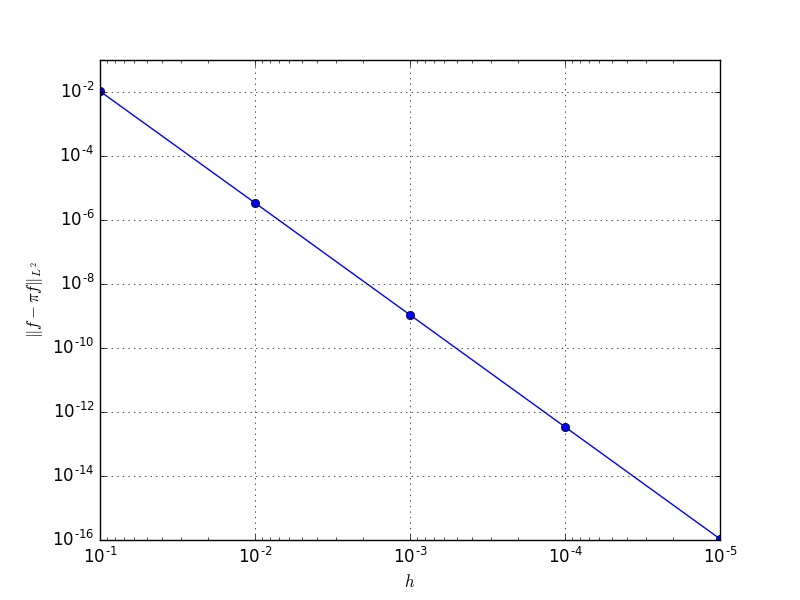
\includegraphics[width=0.8\textwidth]{./cap_mef1d/dados/ex_esterro_interp_lin/ex_esterro_interp_lin}
%     \caption{Erro de interpolação de $f(x)=3\sen(2\pi x)$ no espaço $P_1([0, h])$.}
%     \label{fig:ex_esterro_interp_lin}
%   \end{figure}

% \ifispython
% Com o \fenics, podemos computar os erros de interpolação com o seguinte \href{https://github.com/phkonzen/notas/blob/master/src/MetodoElementosFinitos/cap_mef1d/dados/ex_esterro_interp_lin/ex_esterro_interp_lin.py}{código}:
% \verbatiminput{./cap_mef1d/dados/ex_esterro_interp_lin/ex_esterro_interp_lin.py}
% \fi
% \end{ex}


Vamos, agora, generalizar o resultado da Proposição \ref{prop:interp_lin} para a interpolação no espaço $V_h$ das funções lineares por parte.

% \begin{ex}\label{ex:interp_linpartes}
%   A Figura~\ref{fig:ex_interp_linpartes} ilustra a interpolação da função $f(x)=3\sen(2\pi x)$ no espaço $V_h$ das funções lineares por partes em uma malha uniforme do intervalo $I=[1/4, 3/4]$ com $n=4$ subintervalos ($5$ pontos). 

%   \begin{figure}[h!]
%     \centering
%     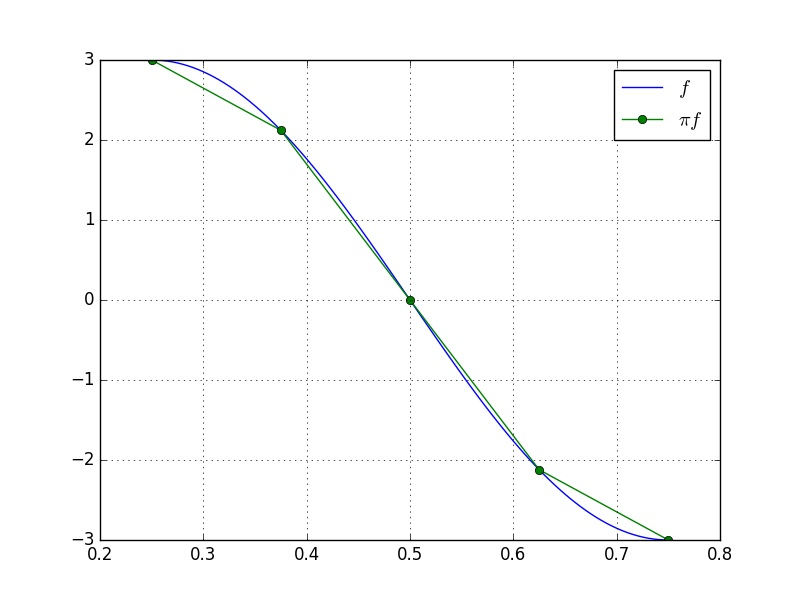
\includegraphics[width=0.8\textwidth]{./cap_mef1d/dados/ex_interp_linpartes/ex_interp_linpartes}
%     \caption{Interpolação linear de $f(x)=3\sen(2\pi x)$ no espaço $V_h$ das funções lineares por partes sobre uma malha com $5$ pontos.}
%     \label{fig:ex_interp_linpartes}
%   \end{figure}

% \ifispython
% Com o \fenics, podemos computar a função interpolada $\pi f$ com o seguinte \href{https://github.com/phkonzen/notas/blob/master/src/MetodoElementosFinitos/cap_mef1d/dados/ex_interp_linpartes/ex_interp_linpartes.py}{código}:
% \verbatiminput{./cap_mef1d/dados/ex_interp_linpartes/ex_interp_linpartes.py}
% \fi
% \end{ex}

O seguinte resultado fornece uma estimativa do erro de interpolação em relação ao tamanho $h_i$ de cada elemento da malha.

\begin{prop}\label{prop:interp_linpartes}
  O interpolador $\pi f$ satisfaz as estimativas
  \begin{align}
    \|f-\pi f\|_{L^2(I)}^2 &\leq C\sum_{i=1}^n h_i^4\|f''\|_{L^2(I)}^2,\\
    \|(f-\pi f)'\|_{L^2(I)}^2 &\leq C\sum_{i=1}^n h_i^2\|f''\|_{L^2(I)}^2.\\
  \end{align}
\end{prop}
\begin{dem}
  Ambas desigualdades seguem da desigualdade triangular e da Proposição~\ref{prop:interp_lin}. Por exemplo, para a primeira desigualdade, temos
  \begin{align}
    \|f - \pi f\|_{L^2(I)}^2 &\leq \sum_{i=1}^n \|f - \pi f\|_{L^2(I_i)}^2\\
    &\leq \sum_{i=1}^n Ch_i^4 \|f''\|_{L^2(I_i)}^2.
  \end{align}
\end{dem}

\subsection{Projeção $L^2$}\label{subsec:projecao_1d}
[[tag:revisar]]

Dada uma função $f\in L^2(I)$, definimos o \hlemph{operador de projeção $L^2$} $P_h:L^2(I)\to V_h$ por
\begin{equation}\label{eq:proj_def}\hleq
  \int_I (f-P_hf)v\,dx=0,\quad\forall v\in V_h.
\end{equation}

Como $V_h$ é um espaço de dimensão finita, a condição \eqref{eq:proj_def} é equivalente a
\begin{equation}\label{eq:proj_def}
  \int_I (f-P_hf)\varphi_i\,dx=0,\quad i=0, 1, \cdots, n,
\end{equation}
onde $\varphi_i$ é a $i$-ésima função base de $V_h$. Além disso, como $P_hf\in V_h$, temos
\begin{equation}
  P_hf = \sum_{j=0}^n\xi_j\varphi_j,
\end{equation}
onde $\xi_j$, $j=0, 1, \dotsc, n$, são $n+1$ incógnitas a determinar. Logo,
\begin{gather}
  \int_I (f-P_hf)\varphi_i\,dx=0 \\
  \int_I f\varphi_i\,dx = \int_I P_hf\varphi_i\,dx\\
  \int_I f\varphi_i\,dx = \int_I \left(\sum_{j=0}^n \xi_j\varphi_j\right)\varphi_i\,dx\\
  \sum_{j=0}^n \xi_j\int_I\varphi_j\varphi_i\,dx = \int_I f\varphi_i\,dx,\label{eq:proj_siseq}
\end{gather}
para $i=0, 1, \dotsc, n$.

Observamos que \eqref{eq:proj_siseq} consiste em um sistema de $n+1$ equações lineares para as $n+1$ incógnitas $\xi_j$, $j=0, 1, \dotsc, n$. Este, por sua vez, pode ser escrito na seguinte forma matricial
\begin{equation}\label{eq:proj_sis}\hleq
  M\xi = b,
\end{equation}
onde \hl{$M = [m_{i,j}]_{i,j=0}^{n+1}$ é chamada de \emph{matriz de massa}}
\begin{equation}\hleq
  m_{i,j} = \int_I\varphi_j\varphi_i\,dx
\end{equation}
e \hl{$b = (b_0, b_1, \dotsc, b_n)$ é chamado de \emph{vetor de carregamento}}
\begin{equation}\hleq
  b_i = \int_I f\varphi_i\,dx.
\end{equation}

Ou seja, \hl{a projeção $L^2$ de $f$ no espaço $V_h$ é}
\begin{equation}\hleq
  P_hf = \sum_{j=0}^n\xi_j\varphi_j,
\end{equation}
\hl{onde $\xi = (\xi_0, \xi_1, \dotsc, \xi_n)$ é solução do sistema {\eqref{eq:proj_sis}}}.

\begin{ex}\label{ex:mef1d_proj}
  A Figura~\ref{fig:ex_mef1d_proj} ilustra a projeção $L^2$ da função $f(x)=3\sen(2\pi x)$ no espaço $V_h$ das funções lineares por partes em uma malha uniforme do intervalo $I=[1/4, 3/4]$ com $n=4$ subintervalos ($5$ células).

  \begin{figure}[h!]
    \centering
    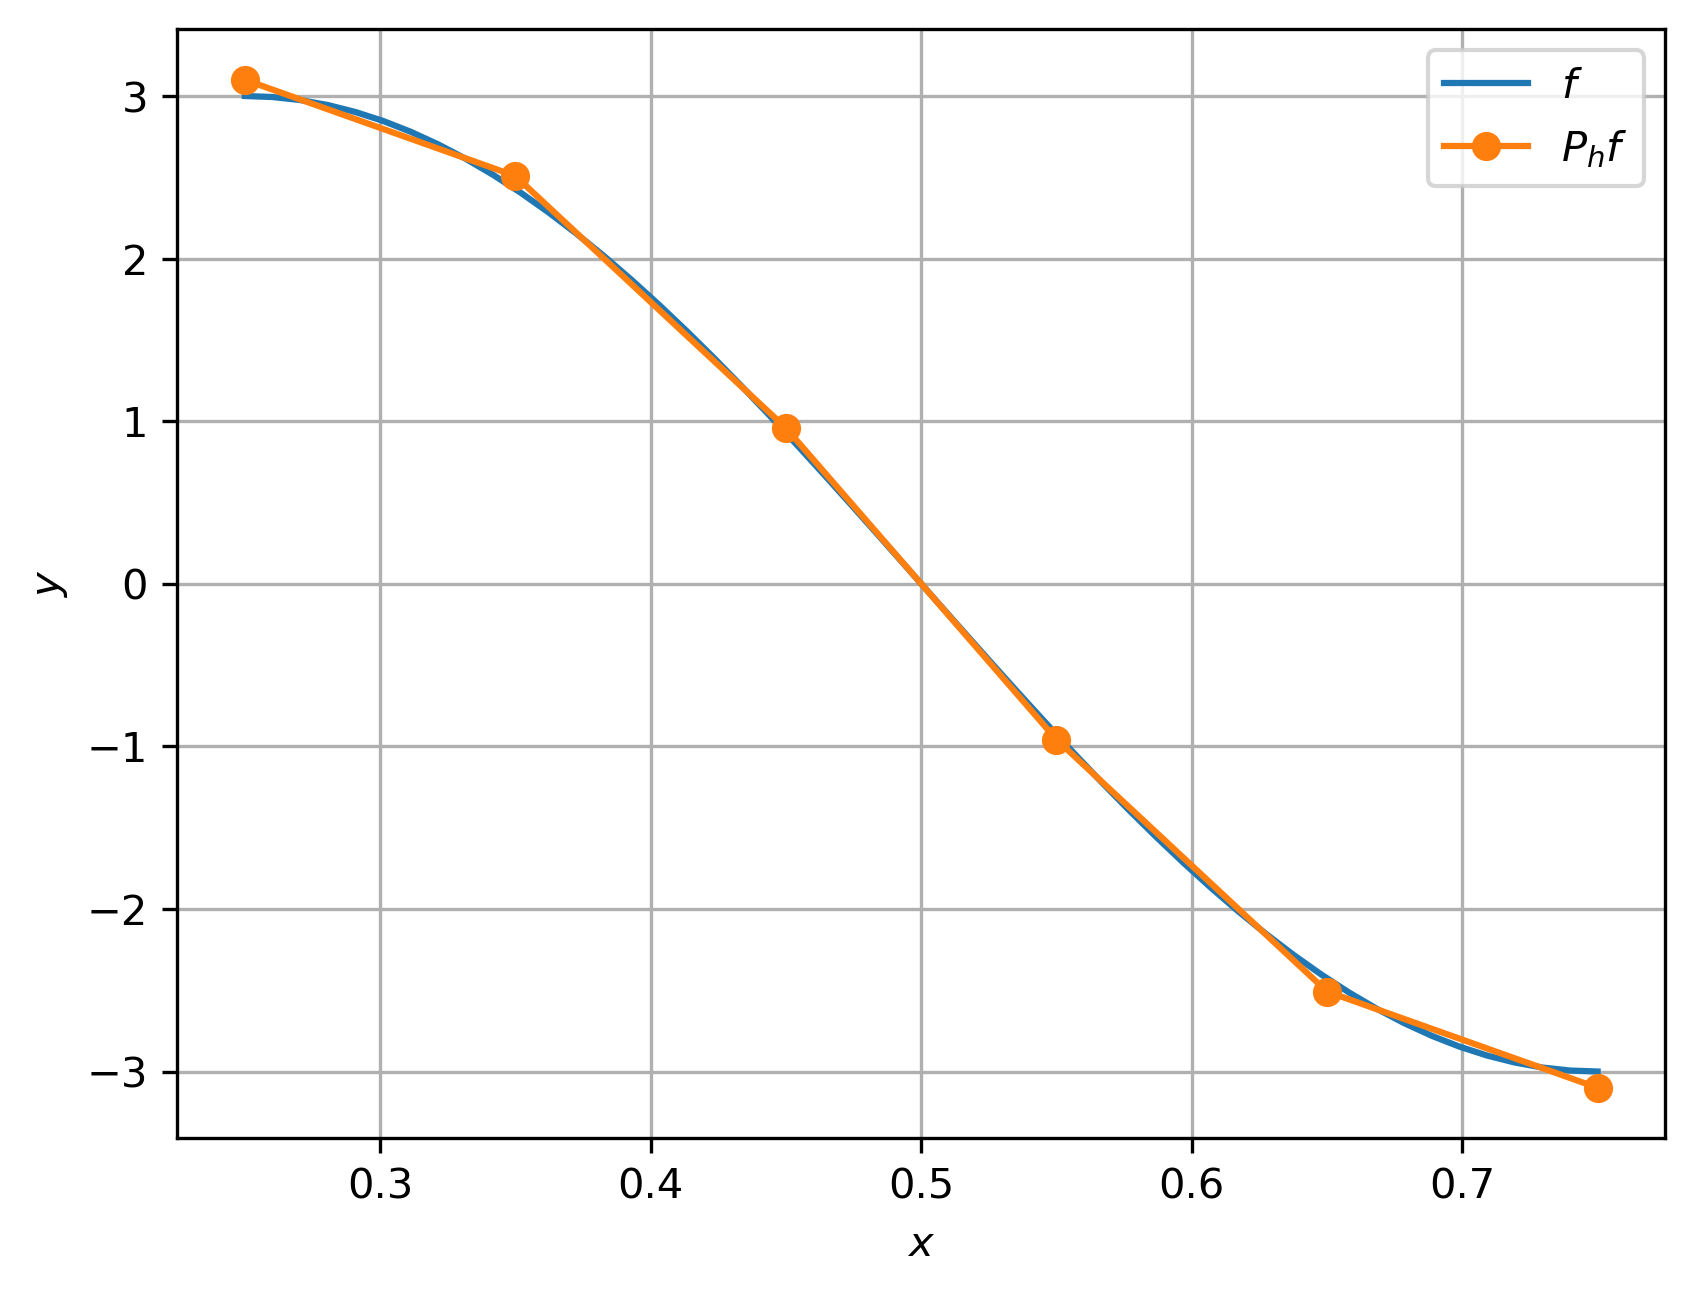
\includegraphics[width=0.8\textwidth]{./cap_mef1d/dados/ex_mef1d_proj/fig}
    \caption{Projeção $L^2$ de $f(x)=3\sen(2\pi x)$ no espaço $V_h$ das funções lineares por partes sobre uma malha com $5$ células.}
    \label{fig:ex_mef1d_proj}
  \end{figure}

\begin{lstlisting}[caption=ex\_mef1d\_proj.py]
from dolfinx import fem, mesh
from dolfinx.fem.petsc import LinearProblem
import ufl
from mpi4py import MPI

# malha
l0 = 0.25
l1 = 0.75
domain = mesh.create_interval(MPI.COMM_WORLD,
                              nx=5,
                              points=[l0, l1])
x = ufl.SpatialCoordinate(domain)

# espaço
V = fem.functionspace(domain, ("P", 1))

# fun
f = 3.*ufl.sin(2.*ufl.pi*x[0])

# project f
u = ufl.TrialFunction(V)
v = ufl.TestFunction(V)
a =  ufl.dot(u, v) * ufl.dx
L = ufl.dot(f, v) * ufl.dx
problem = LinearProblem(a, L, bcs=[])
Phf = problem.solve()
\end{lstlisting}
\end{ex}

O próximo teorema mostra que $P_h f$ é a função que melhor aproxima $f$ dentre todas as funções do espaço $V_h$.

\begin{teo}(\normalfont{A melhor aproximação.})\label{teo:melhor_aprox}
  A projeção $L^2$ satisfaz
  \begin{equation}
    \|f-P_hf\|_{L^2(I)} \leq \|f - v\|_{L^2(I)},\quad\forall v\in V_h.
  \end{equation}
\end{teo}
\begin{dem}
  Dado $v\in V_h$, temos
  \begin{align}
    \|f-P_hf\|_{L^2(I)}^2 &= \int_I |f-P_hf|^2\,dx\\
    &= \int_I (f-P_hf)(f-v+v-P_hf)\,dx\\
    &= \int_I(f-P_hf)(f-v)\,dx + \int_I(f-P_hf)(v-P_hf)\,dx\\
    &= \int_I (f-P_hf)(f-v)\,dx\\
    &\leq \|f-P_hf\|_{L^2(I)}\|f-v\|_{L^2(I)},
  \end{align}
donde segue o resultado.
\end{dem}

O próximo teorema fornece uma estimativa {\it a-priori} do erro $\|f-P_h f\|_{L^2(I)}$ em relação ao tamanho da malha.

\begin{teo}\label{teo:erro_proj_1d}
  A projeção $L^2$ satisfaz
  \begin{equation}
    \|f-P_hf\|_{L^2(I)}^2 \leq C\sum_{i=1}^n h_i^4\|f''\|_{L^2(I_i)}^2.
  \end{equation}
\end{teo}
\begin{dem}
  Tomando a interpolação $\pi f \in V_h$, temos do Teorema da melhor aproximação (Teorema \ref{teo:melhor_aprox}) e da estimativa do erro de interpolação (Proposição \ref{prop:interp_linpartes}) que
  \begin{align}
    \|f - P_hf\|_{L^2(I)}^2 &\leq \|f-\pi f\|_{L^2(I)}^2\\
    &\leq C\sum_{i=1}^n h_i^4\|f''\|_{L^2(I_i)}^2.
  \end{align}
\end{dem}

% \begin{ex}\label{ex:esterro_proj}
%   A Figura \ref{fig:ex_esterro_proj} mostra a evolução do erro na norma $L^2$ da projeção de $f(x)=3\sen(2\pi x)$ no espaço $V_h$ em malhas uniformes de $h=10^{-5}, 10^{-4}, \cdots, 10^{-1}$ no intervalo $[1/4, 3/4]$.

%   \begin{figure}[h!]
%     \centering
%     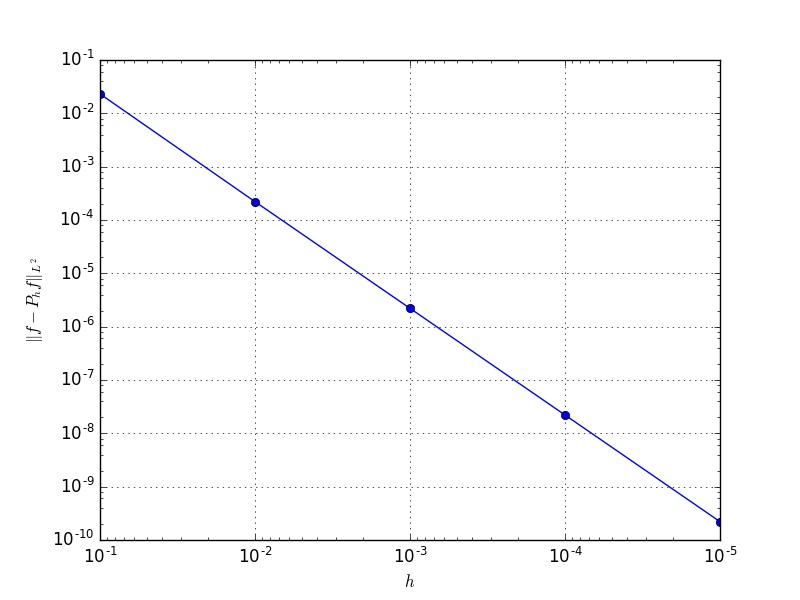
\includegraphics[width=0.8\textwidth]{./cap_mef1d/dados/ex_esterro_proj/ex_esterro_proj}
%     \caption{Erro de interpolação de $f(x)=3\sen(2\pi x)$ no espaço $V_h$.}
%     \label{fig:ex_esterro_proj}
%   \end{figure}

% \ifispython
% Com o \fenics, podemos computar os erros de projeção com o seguinte \href{https://github.com/phkonzen/notas/blob/master/src/MetodoElementosFinitos/cap_mef1d/dados/ex_esterro_proj/ex_esterro_proj.py}{código}:
% \verbatiminput{./cap_mef1d/dados/ex_esterro_proj/ex_esterro_proj.py}
% \fi
% \end{ex}

\subsection{Exercícios}
[[tag:revisar]]

\begin{exer}
  Faça um código para verificar a segunda estimativa da Proposição~\ref{prop:interp_lin} no caso da interpolação da função $f(x) = 3\sen(2\pi x)$ no espaço $P_1$ das funções lineares.
\end{exer}


\begin{exer}
  Faça um código para verificar as estimativas da Proposição~\ref{prop:interp_linpartes} no caso da interpolação da função $f(x) = 3\sen(2\pi x)$ no espaço $V_h$ das funções lineares por partes.
\end{exer}

\begin{exer}
  Faça um código para computar a projeção $L^2$ $P_hf$ da função $f(x) = x - cos(x)$ no espaço $V_h$ das funções lineares por partes em uma malha com $10$ células no intervalo $I = [0, \pi]$. Faça o esboço dos gráficos de $f$ e $P_hf$ e compute o erro $\|f-P_hf\|_{L^2(I)}$.
\end{exer}

\section{Problema modelo}\label{cap_mef1d_sec_modelo}
[[tag:revisar]]

Nesta seção, discutimos sobre a aplicação do método de elementos finitos para o seguinte problema de valor de contorno: encontrar $u$ tal que
\begin{align}
  -u'' &= f,\quad x\in I=[0,L],\label{eq:prob_eq}\\
  u(0) &= u(L) = 0,\label{eq:prob_bc}
\end{align}
onde $f$ é uma função dada.

\subsection{Formulação fraca}
[[tag:revisar]]

A derivação de um método de elementos finitos inicia-se da formulação fraca do problema em um espaço de funções apropriado. No caso do problema \eqref{eq:prob_eq}-\eqref{eq:prob_bc}, tomamos o espaço
\begin{equation}
  V_0 = \{v\in H^1(I):~v(0)=v(1)=0\}.
\end{equation}
Ou seja, se $v\in H^1(I)$, então $\|v\|_{L^2(I)}<\infty$, $\|v'\|_{L^2(I)}<\infty$, bem como $v$ satisfaz as condições de contorno do problema.

A formulação fraca é, então, obtida multiplicando-se a equação \eqref{eq:prob_eq} por uma função teste $v\in V_0$ (arbitrária) e integrando-se por partes, i.e.
\begin{align}
  \int_I fv\,dx &= -\int_I u''v\,dx\\
  &= \int_I u'v'\,dx - u'(L)v(L) + u'(0)v(0)\\
\end{align}
Donde, das condições de contorno, temos
\begin{equation}
  \int_I u'v'\,dx = \int_I fv\,dx.
\end{equation}

Desta forma, o problema fraco associado a \eqref{eq:prob_eq}-\eqref{eq:prob_bc} lê-se: encontrar $u\in V_0$ tal que
\begin{equation}\label{eq:modelo_ffraca}
  a(u,v) = L(v),\quad\forall v\in V_0,
\end{equation}
onde
\begin{align}
  a(u,v) &= \int_I u'v'\,dx\label{eq:modelo_fbilinear}\\
  L(v) &= \int_I fv\,dx,\label{eq:modelo_flinear}
\end{align}
são chamadas de forma bilinear e forma linear, respectivamente.

\subsection{Formulação de elementos finitos}
[[tag:revisar]]

Uma formulação de elementos finitos é um aproximação do problema fraco \eqref{eq:modelo_ffraca} em um espaço de dimensão finita. Aqui, vamos usar o espaço $V_{h,0}$ das funções lineares por partes em $I$ que satisfazem as condições de contorno, i.e.
\begin{equation}
  V_{h,0} = \{v\in V_h:~v(0)=v(L)=0\}.
\end{equation}

Então, substituindo o espaço $V_0$ pelo subespaço $V_{h,0}\subset V_0$ em \eqref{eq:modelo_ffraca}, obtemos o seguinte problema de elementos finitos: encontrar $u_h\in V_{h,0}$ tal que
\begin{equation}\label{eq:modelo_fem}
  a(u_h,v) = L(v),\quad\forall v\in V_{h,0}.
\end{equation}

\begin{obs}
  A formulação de elementos finitos não é única, podendo-se trabalhar com outros espaços de funções. No caso em que o espaço da solução é igual ao espaço das funções testes, a abordagem é chamada de método de Galerkin\footnote{Boris Grigoryevich Galerkin, matemático e engenheiro soviético. Fonte: \href{https://pt.wikipedia.org/wiki/Boris_Galerkin}{Wikipédia}.}.
\end{obs}

Observemos que o problema \eqref{eq:modelo_fem} é equivalente a: encontrar $u_h\in V_{h,0}$ tal que
\begin{equation}
  a(u_h,\varphi_i) = L(\varphi_i),\quad i=1, \dotsc, n-1,
\end{equation}
onde $\varphi_i$, $i=1,\dotsc,n-1$, são as funções base de $V_{h,0}$. Então, como $u_h\in V_{h,0}$, temos
\begin{equation}
  u_h = \sum_{j=1}^{n-1}\xi_j\varphi_j,
\end{equation}
onde $\xi_j$, $j=1,2,\dotsc,n-1$, são incógnitas a determinar. I.e., ao computarmos $\xi_j$, $j=1,2,\dotsc,n-1$, temos obtido a solução $u_h$ do problema de elementos finitos \ref{eq:modelo_fem}.

Agora, da forma bilinear \eqref{eq:modelo_fbilinear}, temos
\begin{align}
  a(u_h,\varphi_i) &= a\left(\sum_{j=1}^{n-1}\xi_j\varphi_j,\varphi_i\right)\\
  &= \sum_{j=1}^{n-1}\xi_j a(\varphi_j,\varphi_i).
\end{align}

Daí, o problema \eqref{eq:modelo_fem} é equivalente a resolvermos o seguinte sistema de equações lineares
\begin{equation}\label{eq:modelo_fem_sis}
  A\xi = b,
\end{equation}
onde $A = [a_{i,j}]_{i,j=1}^{n-1}$ é a matriz de rigidez com
\begin{equation}
  a_{i,j} = a(\varphi_j,\varphi_i) = \int_{I}\varphi_j'\varphi_i'\,dx,
\end{equation}
$\xi = (\xi_1,\xi_2,\dotsc,\xi_{n-1})$ é o vetor das incógnitas e $b = (b_{i})_{i=1}^{n-1}$ é o vetor de carregamento com
\begin{equation}
  b_i = L(\varphi_i) = \int_If \varphi_i\,dx.
\end{equation}

\begin{ex}\label{ex:mef1d_modelo}
  Consideremos o problema \eqref{eq:prob_eq}-\eqref{eq:prob_bc} com $f\equiv 1$ e $L=1$, i.e.
  \begin{align}
    -u'' &= 1,\quad x\in I=[0,1],\label{eq:ex_modelo_eq}\\
    u(0) &= u(1) = 0.\label{eq:ex_modelo_bc}
  \end{align}
Neste caso, a solução analítica $u(x) = -x^2/2+x/2$ pode ser facilmente obtida por integração.

Agora, vamos computar uma aproximação de elementos finitos no espaço das funções lineares por partes $V_{h,0} = \{v\in P_1(I);~v(0)=v(1)=0\}$ construído numa malha uniforme de $5$ células no intervalo $I=[0, 1]$. Para tanto, consideramos o problema fraco: encontrar $u\in V_0 = \{v\in H^1(I);~v(0)=v(L)=0\}$ tal que
\begin{equation}
  a(u, v) = L(v),
\end{equation}
onde
\begin{equation}
  a(u, v) = \int_I u'v'\,dx,\quad L(v)=\int_I fv\,dx.
\end{equation}

Então, a formulação de elementos finitos associada, lê-se: encontrar $u_h\in V_{h,0}$ tal que
\begin{equation}
  a(u_h, v_h) = L(v_h),\quad\forall v_h\in V_{h,0}.
\end{equation}
A Figura \ref{fig:ex_modelo} apresenta o esboço dos gráficos da solução analítica $u$ e da sua aproximação de elementos finitos $u_h$.

\begin{figure}[h!]
  \centering
  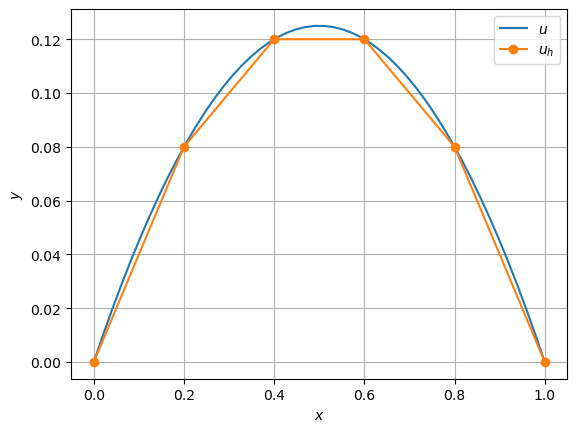
\includegraphics[width=0.8\textwidth]{./cap_mef1d/dados/ex_mef1d_modelo/fig}
  \caption{Esboço dos gráficos das soluções referentes ao Exemplo~\ref{ex:mef1d_modelo}.}
  \label{fig:ex_mef1d_modelo}
\end{figure}

\begin{lstlisting}[caption=ex\_mef1d\_modelo.py]
from mpi4py import MPI

# malha
from dolfinx import mesh
domain = mesh.create_unit_interval(MPI.COMM_WORLD,
                                   nx = 5)
# espaço
from dolfinx import fem
V = fem.functionspace(domain, ('P', 1))

# condição de contorno
import numpy as np
uD = fem.Function(V)
uD.interpolate(lambda x: np.full(x.shape[1], 0.))

tdim = domain.topology.dim
fdim = tdim - 1
domain.topology.create_connectivity(fdim, tdim)
boundary_facets = mesh.exterior_facet_indices(domain.topology)
boundary_dofs = fem.locate_dofs_topological(V, fdim,
                                            boundary_facets)
bc = fem.dirichletbc(uD, boundary_dofs)

# problema mef
import ufl
from dolfinx import default_scalar_type
from dolfinx.fem.petsc import LinearProblem
u = ufl.TrialFunction(V)
v = ufl.TestFunction(V)

f = fem.Constant(domain, default_scalar_type(1.))

a = ufl.dot(ufl.grad(u), ufl.grad(v)) * ufl.dx
L = f * v * ufl.dx

problem = LinearProblem(a, L, bcs=[bc])
uh = problem.solve()
\end{lstlisting}
\end{ex}

\subsection{Estimativa {\it a priori}}
[[tag:revisar]]

Existem dois tipos de estimativas do erro $e := u - u_h$. Estimativas {\it a priori}, são aqueles em que o erro é dado em relação da solução $u$, enquanto que nas estimativas {\it a posteriori} o erro é expresso em relação a solução de elementos finitos $u_h$.

\begin{teo}(\normalfont{Ortogonalidade de Galerkin})\label{teo:ortogonalidade_de_Galerkin}
  A solução de elementos finitos $u_h$ de \eqref{eq:modelo_fem} satisfaz a seguinte propriedade de ortogonalidade
  \begin{equation}
    a(u-u_h,v) := \int_I (u-u_h)'v'\,dx = 0,\quad v\in V_{h,0},
  \end{equation}
onde $u$ é a solução de \eqref{eq:modelo_ffraca}.
\end{teo}
\begin{dem}
  De \eqref{eq:modelo_fem}, \eqref{eq:modelo_ffraca} e lembrando que $V_{h,0}\subset V_0$, temos
  \begin{equation}
    a(u,v) = L(v) = a(u_h,v) \Rightarrow a(u-u_h, v) = 0,
  \end{equation}
para todo $v\in V_{h,0}$.
\end{dem}

\begin{teo}(\normalfont{A melhor aproximação})\label{teo:fem1d_melhor_aprox}
  A solução de elementos finitos $u_h$ dada por \eqref{eq:modelo_fem} satisfaz a seguinte propriedade de melhor aproximação
  \begin{equation}
    \|(u-u_h)'\|_{L^2(I)} \leq \|(u-v)'\|_{L^2(I)},\quad v\in V_{h,0},\label{eq:modelo_melhor_aprox}
  \end{equation}
onde $u$ é a solução de \eqref{eq:modelo_ffraca}.
\end{teo}
\begin{dem}
  Escrevendo $u-u_h = u-v+v-u_h$ para qualquer $v\in V_{h,0}$ e usando a ortogonalidade de Galerkin (Teorema \ref{teo:ortogonalidade_de_Galerkin}), temos
  \begin{align}
    \|(u-u_h)'\|_{L^2(I)}^2 &= \int_{I} (u-u_h)'(u-u_h)'\,dx\\
    &= \int_I (u-u_h)'(u-v+v-u_h)'\,dx\\
    &= \int_I (u-u_h)'(u-v)'\,dx + \int_I (u-u_h)'(v-u_h)'\,dx\\
    &= \int_I (u-u_h)'(u-v)'\,dx\\
    &\leq \|(u-u_h)'\|_{L^2(I)}\|(u-v)'\|_{L^2(I)}.
  \end{align}
\end{dem}

\begin{teo}(\normalfont{Estimativa {\it a priori}})
  O erro em se aproximar a solução $u$ de \eqref{eq:modelo_ffraca} pela solução de elementos finitos $u_h$ dada por \eqref{eq:modelo_fem} satisfaz a seguinte estimativa {\it a priori}
\begin{equation}
  \|(u-u_h)'\|_{L^2(I)}^2 \leq C\sum_{i=1}^n h_i^2\|u''\|_{L^2(I_i)}^2.
\end{equation}
\end{teo}
\begin{dem}
  Tomando $v = \pi u$ no teorema da melhor aproximação (Teorema \ref{teo:fem1d_melhor_aprox}), obtemos
  \begin{equation}
    \|(u-u_h)'\|_{L^2(I)} \leq \|(u-\pi u)'\|_{L^2(I)}.
  \end{equation}
Daí, da estimativa do erro de interpolação (Proposição \ref{prop:interp_linpartes}), temos
\begin{equation}
  \|(u-u_h)'\|_{L^2(I)}^2 \leq C\sum_{i=1}^n h_i^2\|u''\|_{L^2(I_i)}^2.
\end{equation}
\end{dem}

\begin{ex}\label{ex:modelo_estapriori}
  A Figura \ref{fig:ex_modelo_estapriori} apresenta o esboço da evolução do erro $\|(u - u_h)'\|_{L^2(I)}$ da solução de elementos finitos do problema \eqref{eq:ex_modelo_eq}-\eqref{eq:ex_modelo_bc} para malhas uniformes com $n=2, 4, 8, \ldots, 128$ células.

\begin{figure}[h!]
  \centering
  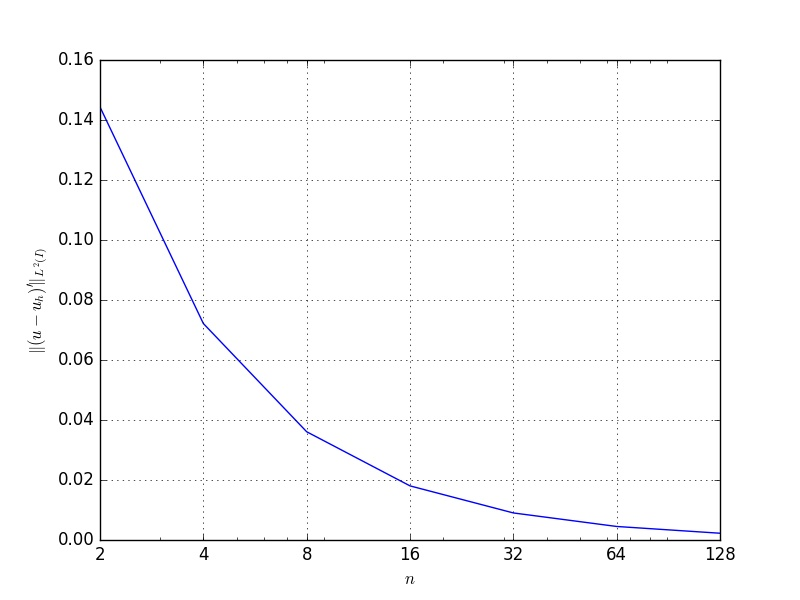
\includegraphics[width=0.8\textwidth]{./cap_mef1d/dados/ex_modelo_estapriori/ex_modelo_estapriori}
  \caption{Esboço dos gráficos das soluções referentes ao Exemplo \ref{ex:modelo_estapriori}.}
  \label{fig:ex_modelo_estapriori}
\end{figure}

\ifispython
Com o \fenics, a computação do problema de elementos finitos pode ser feita com o seguinte \href{https://github.com/phkonzen/notas/blob/master/src/MetodoElementosFinitos/cap_mef1d/dados/ex_modelo_estapriori/ex_modelo_estapriori.py}{código}:
\verbatiminput{./cap_mef1d/dados/ex_modelo_estapriori/ex_modelo_estapriori.py}
\fi
\end{ex}

\subsection{Estimativa {\it a posteriori}}
[[tag:revisar]]

Aqui, vamos obter uma estimativa a posteriori para o erro $e = u - u_h$ da solução de elementos finitos $u_h$ do problema \eqref{eq:prob_eq}-\eqref{eq:prob_bc}.

\begin{teo}\label{teo:fem_est_a_posteriori}
  A solução de elementos finitos $u_h$ satisfaz
  \begin{equation}
    \|(u-u_h)'\|_{L^2(I)}^2 \leq C\sum_{i=1}^n \eta_i^2(u_h),
  \end{equation}
onde $\eta_i(u_h)$ é chamado de elemento residual e é dado por
\begin{equation}
  \eta_i(u_h) = h_i\|f - u_h''\|_{L^2(I_i)}.
\end{equation}
\end{teo}
\begin{dem}
  Tomando $e = u - u_h$ e usando a ortogonalidade de Galerkin (Teorema \ref{teo:ortogonalidade_de_Galerkin}) temos
  \begin{equation}
    \|e'\|_{L^2(I)}^2 = \int_I e'(e-\pi e)'\,dx = \sum_{i=1}^n\int_{I_i} e'(e-\pi e)'\,dx.
  \end{equation}
  Então, aplicando integração por partes
  \begin{equation}
    \|e'\|_{L^2(I)}^2 = \sum_{i=1}^n\int_{I_i}(-e'')(e-\pi e)\,dx + [e'(e-\pi e)]_{x_{i-1}}^{x_i}.
  \end{equation}
  Daí, observando que $e-\pi e = 0$ nos extremos dos intervalos $I_i$ e que $-e'' = -(u-u_h)'' = -u'' + u_h'' = f + u_h''$, temos
  \begin{equation}
    \|e'\|_{L^2(I)}^2 = \sum_{i=1}^n\int_{I_i}(f+u_h'')(e-\pi e)\,dx.
  \end{equation}
  Agora, usando as desigualdades de Cauchy-Schwarz e a estimativa padrão de interpolação \eqref{eq:prop_pif_0}, obtemos
  \begin{align}
    \|e'\|_{L^2(I)}^2 &\leq \sum_{i=1}^n\|f+u_h\|_{L^2(I_i)}\|e-\pi e\|_{L^2(I_i)}\,dx\\
    &\leq C\sum_{i=1}^nh_i\|f+u_h\|_{L^2(I_i)}\|e'\|_{L^2(I_i)}\\
    &\leq C\left(\sum_{i=1}^n h_i^2\|f+u_h\|_{L^2(I_i)}^2\right)^{1/2}\left(\sum_{i=1}^n \|e'\|_{L^2(I_i)}^2\right)^{1/2}\\
    &= C\left(\sum_{i=1}^n h_i^2\|f+u_h\|_{L^2(I_i)}^2\right)^{1/2}\|e'\|_{L^2(I)},
  \end{align}
  donde segue o resultado desejado.
\end{dem}

\begin{obs}
  No caso da solução de elementos finitos no espaço das funções lineares por partes, temos $u_h'' = 0$. Logo, o elemento residual se resume em $\eta_i(u_h) = h_i\|f\|_{L^2(I_i)}$.
\end{obs}

\subsection*{Exercícios}
[[tag:revisar]]

\begin{exer}\label{exer:dc}
  Obtenha uma aproximação por elementos finitos lineares por partes da solução de
  \begin{align}
    &-u'' + u = 2\sen x,\quad \forall x\in (-\pi, \pi),\\
    &u(-\pi)=u(\pi)=0.
  \end{align}
\end{exer}
\begin{resp}
  \ifispython
  \href{https://github.com/phkonzen/notas/blob/master/src/MetodoElementosFinitos/cap_mef1d/dados/exer_dc/exer_dc.py}{Código} FENiCS.
  \fi
\end{resp}


\section{Condições de contorno}\label{cap_mef1d_sec_cc}
[[tag:revisar]]

Nesta seção, vamos discutir sobre soluções de elementos finitos para a equações diferencial
\begin{equation}
  -u'' = f,\quad x\in I=[0, L],
\end{equation}
com diferentes condições de contorno.

\subsection{Condições de Dirichlet}
[[tag:revisar]]

Consideremos o seguinte problema com condições de contorno de Dirichlet\footnote{Johann Peter Gustav Lejeune Dirichlet, 1805 - 1859, matemático alemão. Fonte: \href{https://en.wikipedia.org/wiki/Peter_Gustav_Lejeune_Dirichlet}{Wikipedia}.}: encontrar $u$ tal que
\begin{align}
  &-u'' = f,\quad \forall x\in I=[0, L],\label{eq:cc_d_eq}\\
  &u(0) = u_0,\quad u(L) = u_L,\label{eq:cc_d_bc}
\end{align}
com $u_0$, $u_L$ e $f$ dados.

Tomando uma função teste $v\in V_0=H^1_0(I):=\{v\in H^1(I);~v(0)=v(L)=0\}$ e multiplicando-a em \eqref{eq:cc_d_eq}, obtemos
\begin{equation}
  - \int_I u''v\,dx = \int_I fv\,dx.
\end{equation}
Aplicando a integração por partes, temos
\begin{equation}
  \int_I u'v'\,dx = \int_I fv\,dx.
\end{equation}
Desta forma, definimos o seguinte problema fraco associado: encontrar $u\in V := \{v\in H^1(I);~v(0)=u_0,~v(L)=v_L\}$ tal que
\begin{align}
  a(u,v) = L(v),\quad\forall v\in V_0,
\end{align}
onde $a(u,v)$ é a forma bilinear
\begin{equation}
  a(u,v) = \int_I u'v'\,dx
\end{equation}
e $L(v)$ é a forma linear
\begin{equation}
  L(v) = \int_I fv\,dx.
\end{equation}

\begin{ex}\label{ex:cc_d}
  Consideremos o problema
  \begin{align}
    &-u'' = 1,\quad x\in I=[0,1],\label{eq:ex_cc_d_eq}\\
    &u(0) = 1/2,\quad u(1) = 1.\label{eq:ex_cc_d_bc}
  \end{align}
Sua solução analítica é $u(x) = -x^2/2+x+1/2$. 

Para obtermos uma aproximação de elementos finitos, consideramos o seguinte problema fraco: encontrar $u\in V := \{v\in H^1(I);~v(0)=1/2,~v(1)=1\}$ tal que
\begin{equation}
  a(u,v) = L(v),
\end{equation}
para todo $v\in V_0 = \{v\in H^1(I);~v(0)=v(1)=0\}$, onde
\begin{align}
  a(u, v) &= \int_I u'v'\,dx,\quad L(v) &= \int_I fv\,dx.
\end{align}

Então, o problema de elementos finitos no espaço das funções lineares por partes lê-se: encontrar $u_h\in V_h = \{v\in P_1(I);~v(0)=1/2,~v(1)=1\}$ tal que
\begin{equation}
  a(u_h, v_h) = L(v_h),
\end{equation}
para todo $v_h\in V_{h,0} = \{v\in H^1(I);~v(0)=v(1)=0\}$.

A Figura \ref{fig:ex_cc_d} apresenta o esboço dos gráficos da solução analítica $u$ e da sua aproximação de elementos finitos $u_h$, esta construída no espaço dos polinômios lineares por partes sobre uma malha uniforme de $5$ células.

\begin{figure}[h!]
  \centering
  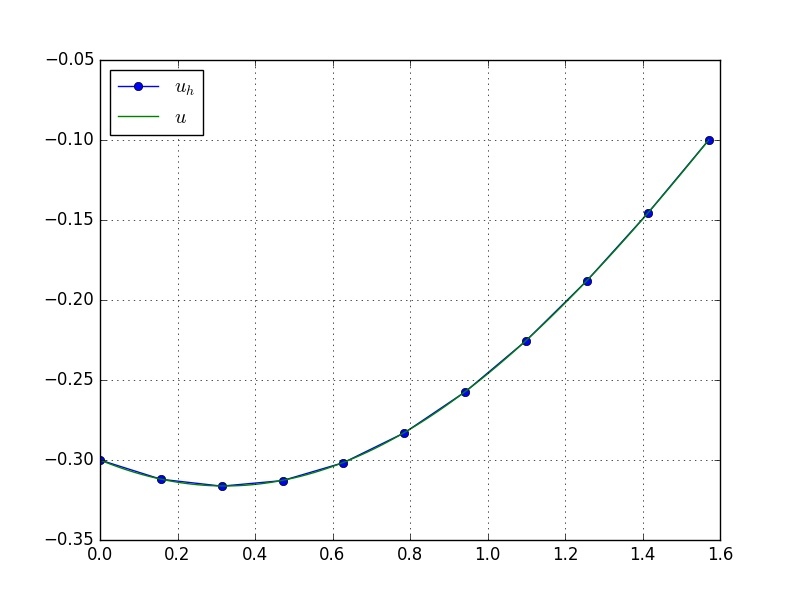
\includegraphics[width=0.8\textwidth]{./cap_mef1d/dados/ex_cc_d/ex_cc_d}
  \caption{Esboço dos gráficos das soluções referentes ao Exemplo \ref{ex:cc_d}.}
  \label{fig:ex_cc_d}
\end{figure}

\ifispython
Com o \fenics, a computação do problema de elementos finitos pode ser feita com o seguinte \href{https://github.com/phkonzen/notas/blob/master/src/MetodoElementosFinitos/cap_mef1d/dados/ex_cc_d/ex_cc_d.py}{código}:
\verbatiminput{./cap_mef1d/dados/ex_cc_d/ex_cc_d.py}
\fi
\end{ex}

\subsection{Condições de Neumann}
[[tag:revisar]]

Consideremos o seguinte problema com condições de contorno de Neumann\footnote{Carl Gottfried Neumann, 1832 - 1925, matemático alemão. Fonte: \href{https://en.wikipedia.org/wiki/Carl_Neumann}{Wikipedia}.} homogênea em $x=L$: encontrar $u$ tal que
\begin{align}
  &-u'' = f,\quad \forall x\in I=[0, L],\label{eq:cc_n_eq}\\
  &u(0) = u_0,\quad u'(L) = 0,\label{eq:cc_n_bc}
\end{align}
com $u_0$ e $f$ dados.

Tomando uma função teste $v\in V:=\{v\in H^1(I);~v(0)=0\}$ e multiplicando-a em \eqref{eq:cc_n_eq}, obtemos
\begin{equation}
  - \int_I u''v\,dx = \int_I fv\,dx.
\end{equation}
Aplicando a integração por partes, temos
\begin{equation}
  \int_I u'v'\,dx - \underbrace{u'(L)v(L)}_{u'(L)=0} + \underbrace{u'(0)v(0)}_{v(0)=0} = \int_I fc\,dx.
\end{equation}
Desta forma, definimos o seguinte problema fraco associado: encontrar $u\in \tilde{V} := \{v\in H^1(I);~v(0)=u_0\}$ tal que
\begin{align}
  a(u,v) = L(v),\quad\forall v\in V,
\end{align}
onde $a(u,v)$ é a forma bilinear
\begin{equation}\label{eq:cc_n_bilinear}
  a(u,v) = \int_I u'v'\,dx
\end{equation}
e $L(v)$ é a forma linear
\begin{equation}\label{eq:cc_n_linear}
  L(v) = \int_I fv\,dx.
\end{equation}

\begin{ex}\label{ex:cc_n}
  Consideremos o problema
  \begin{align}
    &-u'' = 1,\quad x\in I=[0,1],\label{eq:ex_cc_n_eq}\\
    &u(0) = 0,\quad u'(1) = 0.\label{eq:ex_cc_n_bc}
  \end{align}
Sua solução analítica é $u(x) = -x^2/2+x$. 

Podemos construir uma aproximação por elementos finitos do seguinte problema fraco associado: encontrar $u\in V=\{v\in H^1(I);~v(0)=0\}$ tal que
\begin{equation}
  a(u, v) = L(v),
\end{equation}
para todo $v\in V$, com as formas bilinear $a(\cdot, \cdot)$ e linear $L(\cdot)$ dadas em \eqref{eq:cc_n_bilinear} e \eqref{eq:cc_n_linear}.

Então, considerando elementos lineares por partes, temos o seguinte problema de elementos finitos: encontrar $u_h\in V_h=\{v_h\in P_1(I);~v_h(0)=0\}$ tal que
\begin{equation}
  a(u_h, v_h) = L(v_h),\quad\forall v_h\in V_h.
\end{equation}

A Figura \ref{fig:ex_cc_n} apresenta o esboço dos gráficos da solução analítica $u$ e da sua aproximação de elementos finitos $u_h$, esta construída no espaço dos polinômios lineares por partes sobre uma malha uniforme de $5$ células.

\begin{figure}[h!]
  \centering
  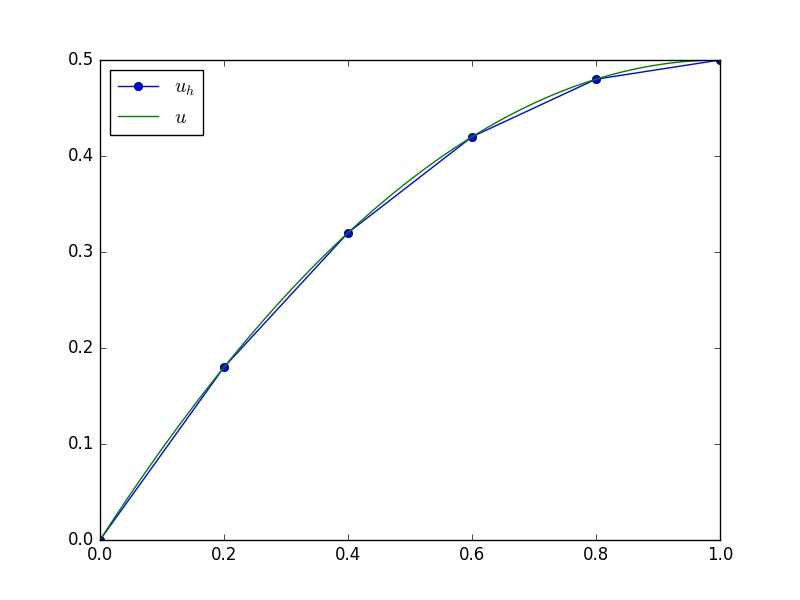
\includegraphics[width=0.8\textwidth]{./cap_mef1d/dados/ex_cc_n/ex_cc_n}
  \caption{Esboço dos gráficos das soluções referentes ao Exemplo \ref{ex:cc_n}.}
  \label{fig:ex_cc_n}
\end{figure}

\ifispython
Com o \fenics, a computação do problema de elementos finitos pode ser feita com o seguinte \href{https://github.com/phkonzen/notas/blob/master/src/MetodoElementosFinitos/cap_mef1d/dados/ex_cc_n/ex_cc_n.py}{código}:
\verbatiminput{./cap_mef1d/dados/ex_cc_n/ex_cc_n.py}
\fi
\end{ex}

Agora, consideremos o seguinte problema com condições de Neumann não-homogênea em $x=L$: encontrar $u$ tal que
\begin{align}
  &-u'' = f,\quad \forall x\in I=[0, L],\label{eq:cc_n2_eq}\\
  &u(0) = u_0,\quad u'(L) = \alpha,\label{eq:cc_n2_bc}
\end{align}
com $u_0$, $\alpha$ e $f$ dados.

Tomando uma função teste $v\in V:=\{v\in H^1(I);~v(0)=0\}$ e multiplicando-a em \eqref{eq:cc_n2_eq}, obtemos
\begin{equation}
  - \int_I u''v\,dx = \int_I fv\,dx.
\end{equation}
Aplicando a integração por partes, temos
\begin{equation}
  \int_I u'v'\,dx - \alpha v(L)= \int_I fc\,dx.
\end{equation}
Desta forma, definimos o seguinte problema fraco associado: encontrar $u\in \tilde{V} := \{v\in H^1(I);~v(0)=u_0\}$ tal que
\begin{align}
  a(u,v) - b( = L(v),\quad\forall v\in V,
\end{align}
onde $a(u,v)$ é a forma bilinear
\begin{equation}
  a(u,v) = \int_I u'v'\,dx
\end{equation}
e $L(v)$ é a forma linear
\begin{equation}
  L(v) = \int_I fv\,dx + \alpha v(L).
\end{equation}

\begin{ex}\label{ex:cc_n2}
  Consideremos o problema
  \begin{align}
    &-u'' = 1,\quad x\in I=[0,1],\label{eq:ex_cc_n2_eq}\\
    &u(0) = 0,\quad u'(1) = 1.\label{eq:ex_cc_n2_bc}
  \end{align}
Sua solução analítica é $u(x) = -x^2/2+2x$. 

Agora, consideramos o seguinte problema fraco associado: encontrar $u\in V=\{v\in H^1(I);~v(0)=0\}$ tal que
\begin{equation}
  a(u,v) = L(v),\quad\forall v\in V,
\end{equation}
com
\begin{equation}
  a(u, v) = \int_I u'v'\,dx
\end{equation}
e
\begin{equation}
  L(v) = \int_I fv\,dx + 1\cdot v(1).
\end{equation}

Então, consideramos o seguinte problema de elementos finitos associado: encontrar $u_h\in V_h = \{v_h\in P_1(I);~v_h(0)=0\}$ tal que
\begin{equation}
  a(u_h, v_h) = L(v_h),\quad\forall v_h\in V_h.
\end{equation}

A Figura \ref{fig:ex_cc_n2} apresenta o esboço dos gráficos da solução analítica $u$ e da sua aproximação de elementos finitos $u_h$, esta construída no espaço dos polinômios lineares por partes sobre uma malha uniforme de $5$ células.

\begin{figure}[h!]
  \centering
  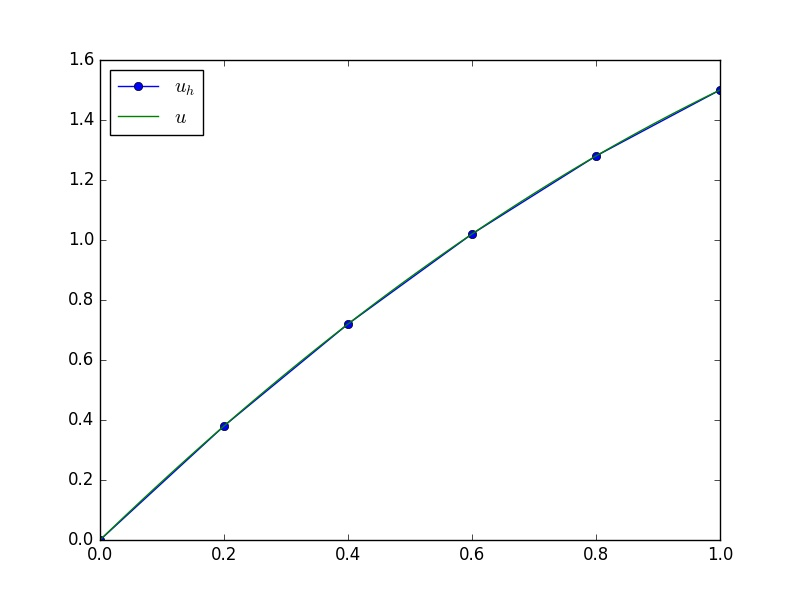
\includegraphics[width=0.8\textwidth]{./cap_mef1d/dados/ex_cc_n2/ex_cc_n2}
  \caption{Esboço dos gráficos das soluções referentes ao Exemplo \ref{ex:cc_n2}.}
  \label{fig:ex_cc_n2}
\end{figure}

\ifispython
Com o \fenics, a computação do problema de elementos finitos pode ser feita com o seguinte \href{https://github.com/phkonzen/notas/blob/master/src/MetodoElementosFinitos/cap_mef1d/dados/ex_cc_n2/ex_cc_n2.py}{código}:
\verbatiminput{./cap_mef1d/dados/ex_cc_n2/ex_cc_n2.py}
\fi
\end{ex} 

\subsection{Condições de Robin}
[[tag:revisar]]

Consideremos o seguinte problema com condições de contorno de Robin\footnote{Victor Gustave Robin, 1855 - 1897, matemático francês. Fonte: \href{https://en.wikipedia.org/wiki/Victor_Robin}{Wikipedia}.}: encontrar $u$ tal que
\begin{align}
  &-u'' = f,\quad \forall x\in I=[0, L],\label{eq:cc_r_eq}\\
  &u'(0) = r_0(u(0)-s_0),~ -u'(L) = r_L(u(L)-s_L),\label{eq:cc_r_bc}
\end{align}
com $r_0$, $r_L$, $s_0$, $s_L$ e $f$ dados.

Tomando uma função teste $v\in V= H^1(I)$ e multiplicando-a em \eqref{eq:cc_r_eq}, obtemos
\begin{equation}
  - \int_I u''v\,dx = \int_I fv\,dx.
\end{equation}
Aplicando a integração por partes, temos
\begin{equation}
  \int_I u'v'\,dx - \underbrace{u'(L)v(L)}_{-u'(L)=r_L(u(L)-s_L)} + \underbrace{u'(0)v(0)}_{u'(0)=r_0(u(0)-s_0)} = \int_I fc\,dx.
\end{equation}
ou, mais adequadamente,
\begin{equation}
  \int_I u'v'\,dx + r_Lu(L)v(L) +r_0u(0)v(0) = \int_I fc\,dx + r_Ls_Lv(L) + r_0s_0v(0).
\end{equation}
Desta forma, definimos o seguinte problema fraco associado: encontrar $u\in H^1(I)$ tal que
\begin{align}
  a(u,v) = L(v),\quad\forall v\in V,
\end{align}
onde $a(u,v)$ é a forma bilinear
\begin{equation}
  a(u,v) = \int_I u'v'\,dx + r_Lu(L)v(L) + r_0u(0)v(0)
\end{equation}
e $L(v)$ é a forma linear
\begin{equation}
  L(v) = \int_I fv\,dx + r_Ls_Lv(L) + r_0s_0v(0).
\end{equation}

\begin{ex}\label{ex:cc_r}
  Consideremos o problema
  \begin{align}
    &-u'' = 1,\quad x\in I=[0,1],\label{eq:ex_cc_r_eq}\\
    &u'(0) = u(0),\quad -u'(1) = u(1) - 1.\label{eq:ex_cc_r_bc}
  \end{align}
Sua solução analítica é $u(x) = -x^2/2+5x/6+5/6$. 

Aqui, tomamos o seguinte problema fraco: encontrar $u\in V=H^1(I)$ tal que
\begin{equation}
  a(u, v) = L(v),\quad\forall v\in V,
\end{equation}
onde
\begin{equation}
  a(u, v) = \int_I u'v'\,dx + u(1)v(1) + u(0)v(0)
\end{equation}
e
\begin{equation}
  L(v) = \int_I fv\,dx + 1\cdot v(1).
\end{equation}

Então, uma aproximação por elementos finitos lineares por partes pode ser obtida resolvendo o seguinte problema: encontrar $u_h\in V_h=P_1(I)$ tal que
\begin{equation}
  a(u_h, v_h) = L(v_h),\quad\forall v_h\in V_h.
\end{equation}

A Figura \ref{fig:ex_cc_r} apresenta o esboço dos gráficos da solução analítica $u$ e da sua aproximação de elementos finitos $u_h$, esta construída no espaço dos polinômios lineares por partes sobre uma malha uniforme de $5$ células.

\begin{figure}[h!]
  \centering
  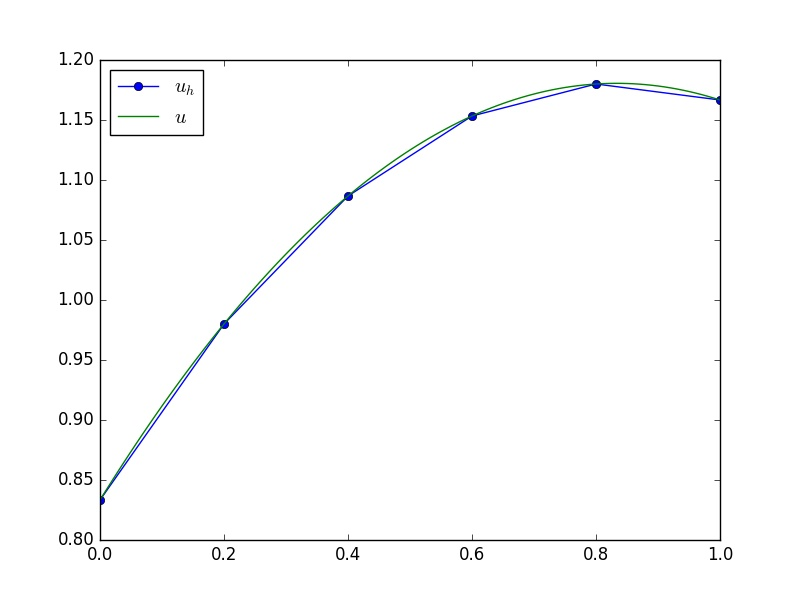
\includegraphics[width=0.8\textwidth]{./cap_mef1d/dados/ex_cc_r/ex_cc_r}
  \caption{Esboço dos gráficos das soluções referentes ao Exemplo \ref{ex:cc_r}.}
  \label{fig:ex_cc_r}
\end{figure}

\ifispython
Com o \fenics, a computação do problema de elementos finitos pode ser feita com o seguinte \href{https://github.com/phkonzen/notas/blob/master/src/MetodoElementosFinitos/cap_mef1d/dados/ex_cc_r/ex_cc_r.py}{código}:
\verbatiminput{./cap_mef1d/dados/ex_cc_r/ex_cc_r.py}
\fi
\end{ex}

\subsection{Exercícios}
[[tag:revisar]]

\begin{exer}\label{exer:dcr}
  Considere o problema
  \begin{align}
    &-u'' + u' + 2u = -\cos(x),\quad x\in (0, \pi/2),\\
    &u(0)=-0,3,\quad u(\pi/2)=-0,1.
  \end{align}
  Obtenha uma aproximação por elementos finitos para a solução deste problema, empregando o espaço de elementos finitos linear sobre uma malha uniforme com $10$ células. Então, compare a aproximação computada com sua solução analítica $u(x) = 0,1(\sen(x)+3\cos(x))$, bem como, compute o erro $\|u-u_h\|_{L^2}$.
\end{exer}
\begin{resp}
  \ifispython
  \href{https://github.com/phkonzen/notas/blob/master/src/MetodoElementosFinitos/cap_mef1d/dados/exer_dcr/exer_dcr.py}{Código}.
  \fi
\end{resp}

\section{Malhas auto-adaptativas}\label{cap_mef1d_sec_adapt}
[[tag:revisar]]

Retornemos ao problema modelo \eqref{eq:prob_eq}-\eqref{eq:prob_bc}
\begin{align}
  -u'' &= f,\quad x\in I=[0,L],\\
  u(0) &= u(L) = 0.
\end{align}
A estimativa {\it a posteriori} dada no Teorema \ref{teo:fem_est_a_posteriori}, indica que os elementos residuais $\eta_i(u_h)$ podem ser utilizados para estimarmos a precisão da aproximação por elementos finitos. Ou seja, espera-se que quanto menores forem os elementos residuais, mais precisa é a solução por elementos finitos. Além disso, como
\begin{equation}
  \eta_i(u_h) = h_i\|f - u_h''\|_{L^2(I_i)},
\end{equation}
podemos reduzir $\eta_i(u_h)$ diminuindo o tamanho da célula $I_i$.

Do observado acima, motiva-se o seguinte algoritmo de elementos finitos com refinamento automático de malha:
\begin{enumerate}
\item Escolhemos uma malha inicial.
\item Iteramos:
  \begin{enumerate}[2.]
  \item Resolvemos o problema de elementos finitos na malha corrente.
  \item Computamos $\eta_i(u_h)$ em cada célula da malha corrente.
  \item Com base na malha corrente, Contruímos uma nova malha pelo refinamento das células com os maiores valores de $\eta_i(u_h)$.
  \item Verificamos o critério de parada.
  \end{enumerate}
\end{enumerate}

Uma estratégia clássica para a escolha das células a serem refinadas é a seguinte: refina-se a $i$-ésima célula se
\begin{equation}\label{eq:ref_estrategia}
  \eta_i(u_h) > \alpha \max_{j=1, 2, \dotsc, n} \eta_j(u_h),
\end{equation}
onde escolhemos $0 < \alpha < 1$.

\begin{ex}\label{ex:modelo_adapt}
  Consideremos o problema
  \begin{align}
    -u'' &= e^{-100|x-\frac{1}{2}|},\quad x\in I=[0,1],\\
    u(0) &= u(1) = 0.
  \end{align}
  Aqui, computamos aproximações de elementos finitos no espaço das funções lineares por partes $V_{h,0} = \{v\in P_1(I);~v(0)=v(1)=0\}$ com sucessivos refinamentos de malha. Utilizamos uma malha inicial uniforme com 10 células e fazemos, então, 5 refinamentos sucessivos utilizando como critério de refinamento a estratégia \eqref{eq:ref_estrategia} com $\alpha = 0,5$. A Figura \ref{fig:ex_modelo_adapt} apresenta o esboço do gráfico da solução de elementos finitos na malha mais refinada. Além disso, na Tabela \ref{tab:ex_modelo_adapt} temos os o número de células e o $\eta_i(u_h)$ máximo respectivo.

\begin{figure}[h!]
  \centering
  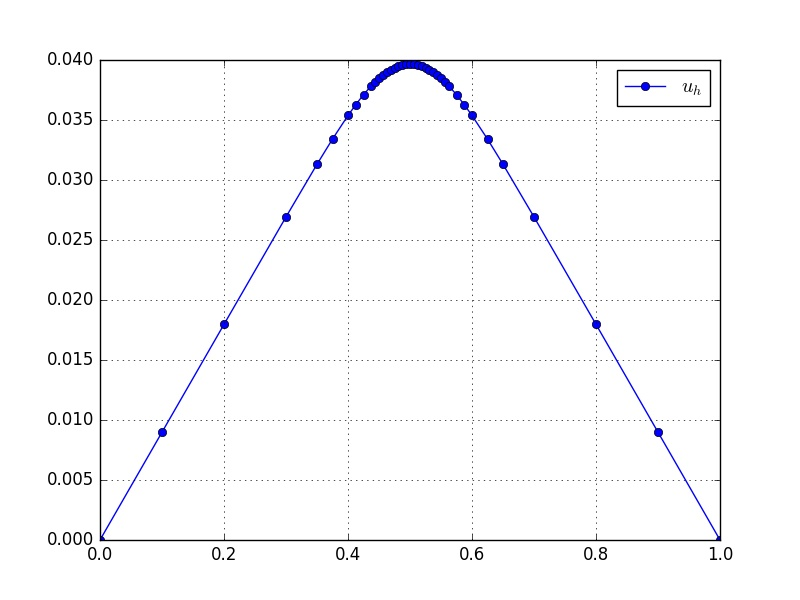
\includegraphics[width=0.8\textwidth]{./cap_mef1d/dados/ex_modelo_adapt/ex_modelo_adapt}
  \caption{Esboço dos gráficos das soluções referentes ao Exemplo \ref{ex:modelo_adapt}.}
  \label{fig:ex_modelo_adapt}
\end{figure}

\begin{table}[h!]
  \centering
  \begin{tabular}{lrc}
    \#malha & \#células & $\max_i\eta_i(u_h)$\\\hline
    0 & 10 & 5.0E-03\\
    1 & 12 & 2.0E-03\\
    2 & 14 & 8.6E-04\\
    3 & 22 & 2.9E-04\\
    4 & 30 & 1.4E-04\\
    5 & 38 & 6.1E-05\\\hline
  \end{tabular}
  \caption{Resultados referente ao Exemplo \ref{ex:modelo_adapt}.}
  \label{tab:ex_modelo_adapt}
\end{table}

\ifispython
Com o \fenics, a computação do problema de elementos finitos pode ser feita com o seguinte \href{https://github.com/phkonzen/notas/blob/master/src/MetodoElementosFinitos/cap_mef1d/dados/ex_modelo_adapt/ex_modelo_adapt.py}{código}:
\verbatiminput{./cap_mef1d/dados/ex_modelo_adapt/ex_modelo_adapt.py}
\fi
\end{ex}

\subsection{Exercícios}
[[tag:revisar]]

\begin{exer}\label{exer:modelo_refglobal}
  Use uma estratégia de sucessivos refinamentos globais para resolver o problema dado no Exemplo \ref{ex:modelo_adapt}. Compare seus resultados com aqueles obtidos no exemplo.
\end{exer}
\begin{resp}
  \ifispython
  \href{https://github.com/phkonzen/notas/blob/master/src/MetodoElementosFinitos/cap_mef1d/dados/exer_dcr/exer_dcr.py}{Código}.
  \fi  
\end{resp}

\section{Seleção de aplicações}\label{cap_mef1d_sec_aps}
[[tag:revisar]]

\subsection{Sistemas de equações}
[[tag:revisar]]

Consideremos o seguinte problema de equações diferenciais ordinárias com valores de contorno
\begin{align}
  &-u_0'' + u_1 = f_0,\forall x\in (0, L)\\ 
  &-u_1'' + u_0 = f_1,\forall x\in (0, L)\\
  &u_0(0)=u_{00},\quad u_0(L)=u_{0L},\\
  &u_1(0)=u_{10},\quad u_1(L)=u_{1L},
\end{align}
onde $f_0$, $f_1$, $u_{00}$, $u_{0L}$, $u_{10}$, $u_{1L}$ são dados.

Para construirmos uma aproximação por elementos finitos podemos tomar o seguinte problema fraco associado: encontrar $u = (u_0, u_1)\in V_0\times V_1$ tal que
\begin{equation}
  a(u, v) = L(v), \forall v = (v_0, v_1)\in V\times V,
\end{equation}
onde $V_0 = \{v\in H^1(I);~v_0(0)=u_{00},~v_0(L)=u_{0L}\}$, $V_1=\{v_1\in H^1(I);~v_1(0)=u_{10},~v_1(L)=u_{1L}\}$, $V = \{v\in H^1(I);~v(0)=v(L)=0\}$, a forma bilinear é
\begin{equation}\label{eq:sis_lin_bilinear}
  a(u, v) = \int_{I} u_0'v_0'\,dx + \int_{I} u_1'v_1'\,dx + \int_{I} u_0v_0\,dx + \int_{I} u_1v_1\,dx
\end{equation}
e a forma linear é
\begin{equation}\label{eq:sis_lin_linear}
  L(v) = \int_I f_0v_0\,dx + \int_I f_1v_1\,dx.
\end{equation}

Então, o problema de elemento finitos associado no espaço das funções lineares por partes lê-se: encontrar $u_h = (u_{h0}, u_{h1})\in V_{h0}\times V_{h1}$ tal que
\begin{equation}
  a(u_h, v_h) = L(v_h), \forall v_h = (v_{h0}, v_{h1})\in V_h\times V_h,
\end{equation}
onde $V_{h0} = \{v_h\in P_1(I);~v_{h0}(0)=u_{00},~v_{h0}(L)=u_{0L}\}$, $V_{h1}=\{v_{h1}\in P_1(I);~v_{h1}(0)=u_{10},~v_{h1}(L)=u_{1L}\}$, $V_h = \{v_h\in P_1(I);~v_h(0)=v_h(L)=0\}$.

\begin{ex}\label{ex:sis_lin}
  Consideremos o seguinte problema de valor de contorno
\begin{align}
  &-u_0'' + u_1 = \sen(x)+\cos(x),\forall x\in (-\pi, \pi)\\ 
  &-u_1'' + u_0 = \cos(x)-\sin(x),\forall x\in (-\pi, \pi)\\
  &u_0(-\pi)=0,\quad u_0(\pi)=0,\\
  &u_1(-\pi)=-1,\quad u_1(\pi)=-1.
\end{align}
Considerando elementos lineares por partes, temos a seguinte formulação de elementos finitos: encontrar $u_h = (u_{h0}, u_{h1})\in V_{h0}\times V_{h1}$ tal que
\begin{equation}
  a(u_h, v_h) = L(v_h), \forall v_h = (v_{h0}, v_{h1})\in V_h\times V_h,
\end{equation}
onde $V_{h0} = \{v_h\in P_1(I);~v_{h0}(0)=v_{h0}(L)=0\}$, $V_{h1}=\{v_{h1}\in P_1(I);~v_{h1}(0)=v_{h1}(L)=-1\}$, $V_h = \{v_h\in P_1(I);~v_h(0)=v_h(L)=0\}$, com as formas bilinear e linear são dadas em \eqref{eq:sis_lin_bilinear} e \eqref{eq:sis_lin_linear}, respectivamente.

A Figura \ref{fig:ex_sis_lin} apresenta o esboço dos gráficos das soluções analíticas $u_0(x)=\sen(x)$ e $u_1(x)=\cos(x)$ e de suas aproximações de elementos finitos $u_{h0}$ e $u_{h1}$, estas construídas no espaço dos polinômios lineares por partes sobre uma malha uniforme de $5$ células.

\begin{figure}[h!]
  \centering
  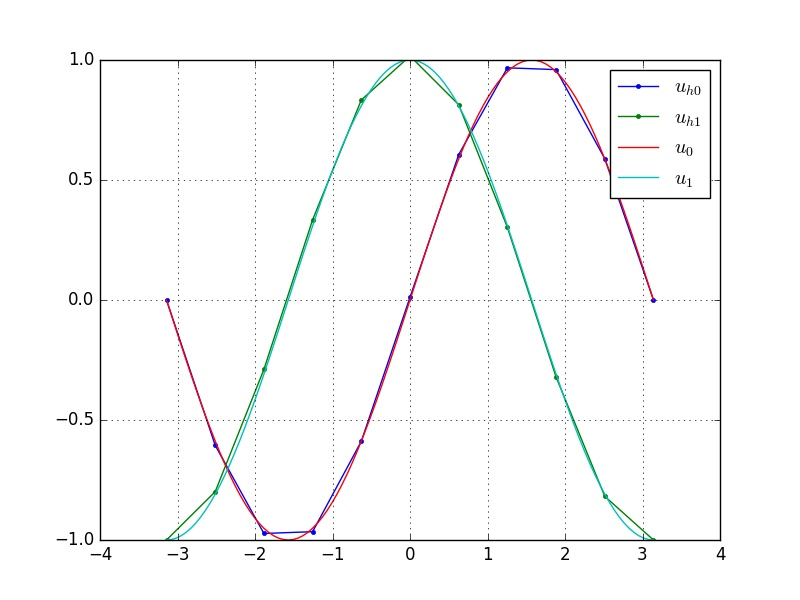
\includegraphics[width=0.8\textwidth]{./cap_mef1d/dados/ex_sis_lin/ex_sis_lin}
  \caption{Esboço dos gráficos das soluções referentes ao Exemplo \ref{ex:sis_lin}.}
  \label{fig:ex_sis_lin}
\end{figure}

\ifispython
Com o \fenics, a computação do problema de elementos finitos pode ser feita com o seguinte \href{https://github.com/phkonzen/notas/blob/master/src/MetodoElementosFinitos/cap_mef1d/dados/ex_sis_lin/ex_sis_lin.py}{código}:
\verbatiminput{./cap_mef1d/dados/ex_sis_lin/ex_sis_lin.py}
\fi
\end{ex}

\subsection{Exercícios}
[[tag:construcao]]

